\subsection*{Problema 16}

\noindent\textbf{Enunciado:} \\
Calcular la integral indefinida:
\begin{align*}
\int \dfrac{x^2 + 1}{x^3 + 1} \, dx
\end{align*}

\noindent\textbf{Solución:} \\
Primero, factorizamos el denominador utilizando la fórmula de la suma de cubos $x^3 + 1 = (x + 1)(x^2 - x + 1)$:
\begin{align*}
\dfrac{x^2 + 1}{x^3 + 1} = \dfrac{x^2 + 1}{(x + 1)(x^2 - x + 1)}
\end{align*}

Aplicamos el método de fracciones parciales planteando la siguiente identidad:
\begin{align*}
\dfrac{x^2 + 1}{(x + 1)(x^2 - x + 1)} = \dfrac{A}{x + 1} + \dfrac{Bx + C}{x^2 - x + 1}
\end{align*}

Multiplicando ambos lados por el denominador común:
\begin{align*}
x^2 + 1 = A(x^2 - x + 1) \\
+ (Bx + C)(x + 1)
\end{align*}

Agrupando términos según las potencias de $x$:
\begin{align*}
x^2 + 1 = (A + B)x^2 \\
+ (-A + B + C)x + (A + C)
\end{align*}

Igualando los coeficientes de ambos lados de la ecuación, obtenemos el sistema:
\begin{align*}
A + B &= 1 \\
-A + B + C &= 0 \\
A + C &= 1
\end{align*}

Resolviendo el sistema, encontramos que:
\begin{align*}
A = \dfrac{2}{3}, \quad B = \dfrac{1}{3}, \quad C = \dfrac{1}{3}
\end{align*}

Sustituyendo los valores en las fracciones parciales, la integral se divide en dos partes:
\begin{align*}
\int \dfrac{x^2 + 1}{x^3 + 1} \, dx = \int \dfrac{2/3}{x + 1} \, dx \\
+ \int \dfrac{\frac{1}{3}x + \frac{1}{3}}{x^2 - x + 1} \, dx
\end{align*}

Resolvemos la primera integral directamente:
\begin{align*}
\int \dfrac{2/3}{x + 1} \, dx = \dfrac{2}{3} \ln|x + 1|
\end{align*}

Para la segunda integral, ajustamos el numerador para que sea la derivada del denominador ($2x - 1$):
\begin{align*}
\int \dfrac{\frac{1}{3}(x + 1)}{x^2 - x + 1} \, dx = \dfrac{1}{6} \int \dfrac{2x + 2}{x^2 - x + 1} \, dx \\
= \dfrac{1}{6} \int \dfrac{(2x - 1) + 3}{x^2 - x + 1} \, dx
\end{align*}

Separamos en dos integrales:
\begin{align*}
= \dfrac{1}{6} \int \dfrac{2x - 1}{x^2 - x + 1} \, dx \\
+ \dfrac{1}{2} \int \dfrac{1}{\left(x - \frac{1}{2}\right)^2 + \frac{3}{4}} \, dx
\end{align*}

La primera se resuelve por sustitución logarítmica y la segunda mediante la fórmula del arco tangente:
\begin{align*}
= \dfrac{1}{6} \ln|x^2 - x + 1| \\
+ \dfrac{1}{2} \left( \dfrac{2}{\sqrt{3}} \arctan\left(\dfrac{2x - 1}{\sqrt{3}}\right) \right)
\end{align*}

Combinando todos los resultados y agregando la constante de integración $C$, la solución general es:
\begin{align*}
\int \dfrac{x^2 + 1}{x^3 + 1} \, dx = \dfrac{2}{3} \ln|x + 1| \\
+ \dfrac{1}{6} \ln|x^2 - x + 1| \\
+ \dfrac{\sqrt{3}}{3} \arctan\left(\dfrac{2x - 1}{\sqrt{3}}\right) + C
\end{align*}

\begin{figure}[H]
	\centering
	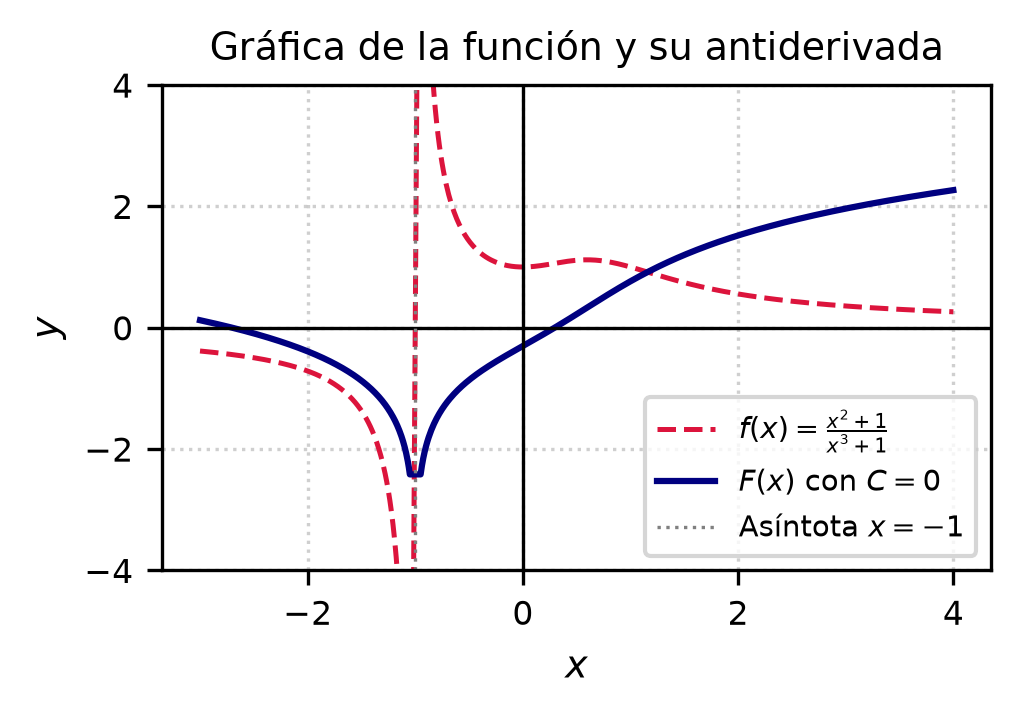
\includegraphics[width=\columnwidth]{semana_03/graficas/SEM03_P16_grafica.png}
	\caption{Representación gráfica de $f(x)$ y su antiderivada $F(x)$ evaluada para la constante de integración $C = 0$ (Problema 16).}
	\label{fig:problema16}
\end{figure}
